\section{Introducción}
En los últimos años, el volumen de contenidos multimedia disponibles en plataformas digitales ha crecido exponencialmente, impulsado por redes sociales, bancos de imágenes, repositorios científicos o plataformas de comercio electrónico. Este crecimiento ha intensificado la necesidad de sistemas eficientes para acceder a dicha información de forma rápida, precisa y alineada con la intención del usuario.

En este contexto, los sistemas de recuperación de información visual, comúnmente conocidos como CBIR (Content-Based Image Retrieval), han supuesto un gran avance, al permitir realizar búsquedas en grandes colecciones de imágenes basándose en características visuales como el color, la forma o la textura. Plataformas ampliamente utilizadas como Google ofrecen funcionalidades como la búsqueda inversa por imagen o sugerencias visuales similares. No obstante, incluso estos sistemas, altamente optimizados, se enfrentan a una limitación crítica: no comprenden el significado profundo de una descripción textual compleja.

Por ejemplo, si un usuario introduce en Google Imágenes la búsqueda: \textit{``niño comiendo caramelos azules''}, los resultados incluyen imágenes de niños comiendo dulces, pero no reflejan de forma precisa todos los elementos descritos. Aparecen niños con piruletas, niños comiendo otros tipos de dulces o con ropa azul, pero no una escena específica con caramelos azules como los que el usuario ha imaginado. Esta limitación es evidente en la Figura~\ref{fig:google_search}.

\begin{figure}[H]
    \centering
    \includegraphics[width=0.9\textwidth]{google.png}
    \caption{Resultados en Google Imágenes}
    \label{fig:google_search}
\end{figure}

Frente a esta limitación, los modelos de inteligencia artificial generativa permiten abordar el problema desde una nueva perspectiva: la generación de contenido visual a partir de texto. En lugar de buscar coincidencias entre imágenes etiquetadas, el sistema genera una imagen completamente nueva que refleja de forma fiel los elementos semánticos de la descripción. En la Figura~\ref{fig:generado}, puede observarse cómo el sistema propuesto ha generado una imagen que representa explícitamente la escena solicitada.

\begin{figure}[ht]
    \centering
    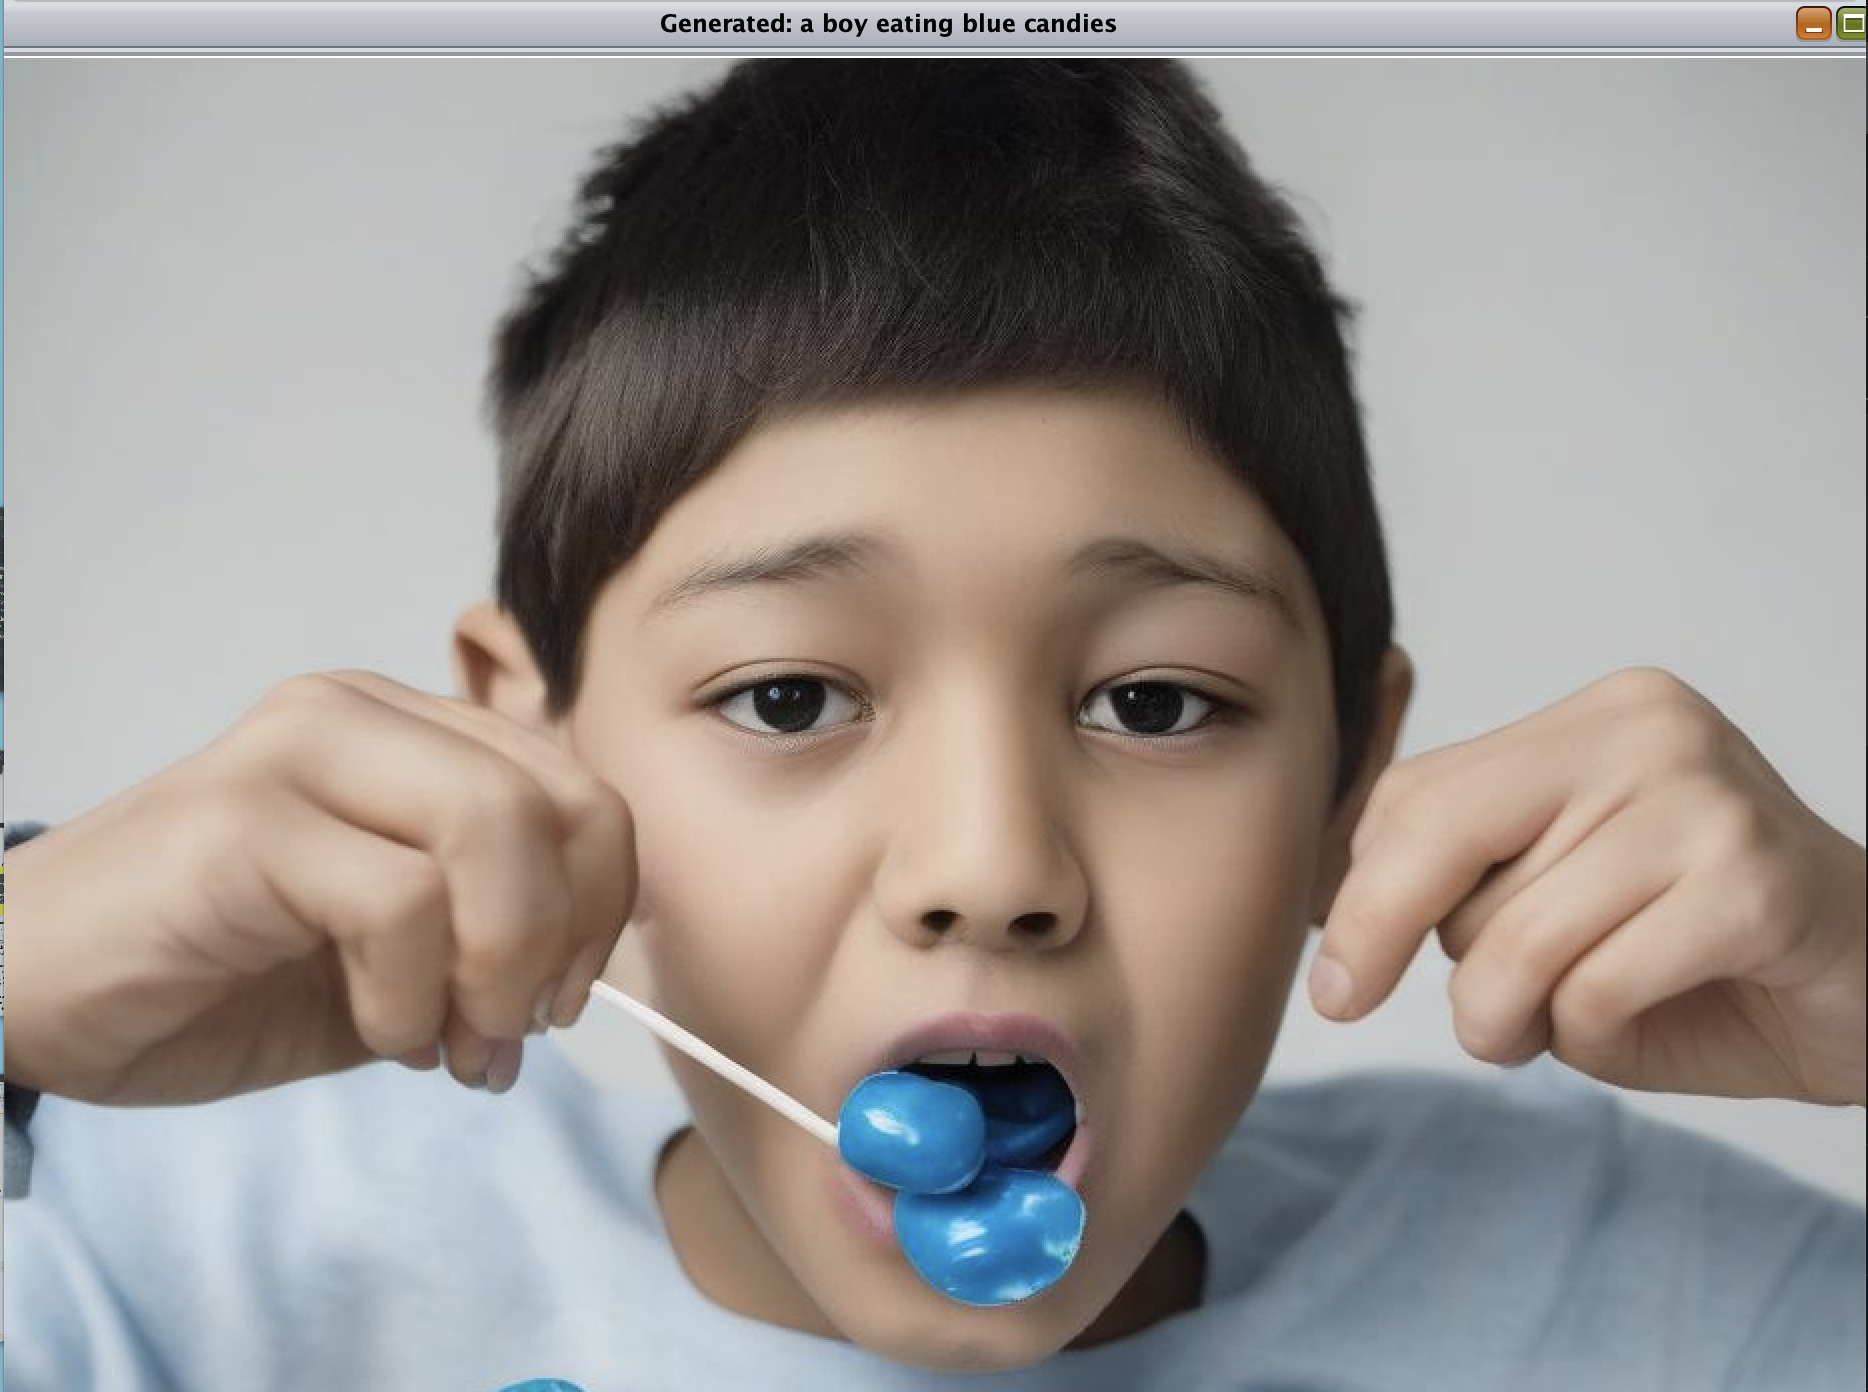
\includegraphics[width=0.5\textwidth]{generated.png}
    \caption{Imagen generada por el sistema propuesto con el prompt: \textit{``a boy eating blue candies''}}
    \label{fig:generado}
\end{figure}

Este proyecto se sitúa en la intersección entre la recuperación visual tradicional y la generación de contenido sintético. Mediante el uso de modelos generativos, se desarrolla un sistema capaz de responder a consultas textuales generando imágenes que actúan como ``consulta visual'', fusionando así lo mejor del CBIR con las capacidades expresivas de la IA generativa. Esta solución se integra dentro de la plataforma Java Multimedia Retrieval (JMR), proporcionando un sistema de recuperación de imágenes más flexible, accesible y centrado en el usuario.

Además del valor técnico, esta tecnología abre nuevas posibilidades para mejorar la accesibilidad en la interacción con sistemas visuales, especialmente para usuarios que no disponen de una imagen de referencia. Poder expresar una búsqueda en lenguaje natural y recibir un resultado visual adecuado representa un avance importante hacia sistemas más inclusivos y adaptativos.

Para validar esta propuesta, se han entrenado y comparado diferentes arquitecturas generativas, se han evaluado sus resultados tanto cualitativa como cuantitativamente, y se ha implementado un prototipo funcional conectado a un sistema de recuperación visual real.

El potencial de este tipo de sistemas va más allá del ámbito académico, con aplicaciones en sectores como la publicidad personalizada, los asistentes creativos, la educación visual o la generación de contenido bajo demanda en plataformas digitales.
